\subsection{UI Interface}

From the system design diagram in Fig.~\ref{fig2b2}, it can be seen that we connect the Flight Controller to the SIK radio and then to the Mission Planner GUI of the computer, we follow this design to setup on the real drone system, the SIK Telemetry Radio devices on the left side of Fig.~\ref{fig2a2}, connected to the Cube Black Flight Controller's Telem Port 1, and the other one is connected to the Laptop's USB port, after initializing the settings in Mission Planner, you can successfully see the monitor screen as shown in Fig.~\ref{fig3e1}.

\begin{figure}[H]
    \centerline{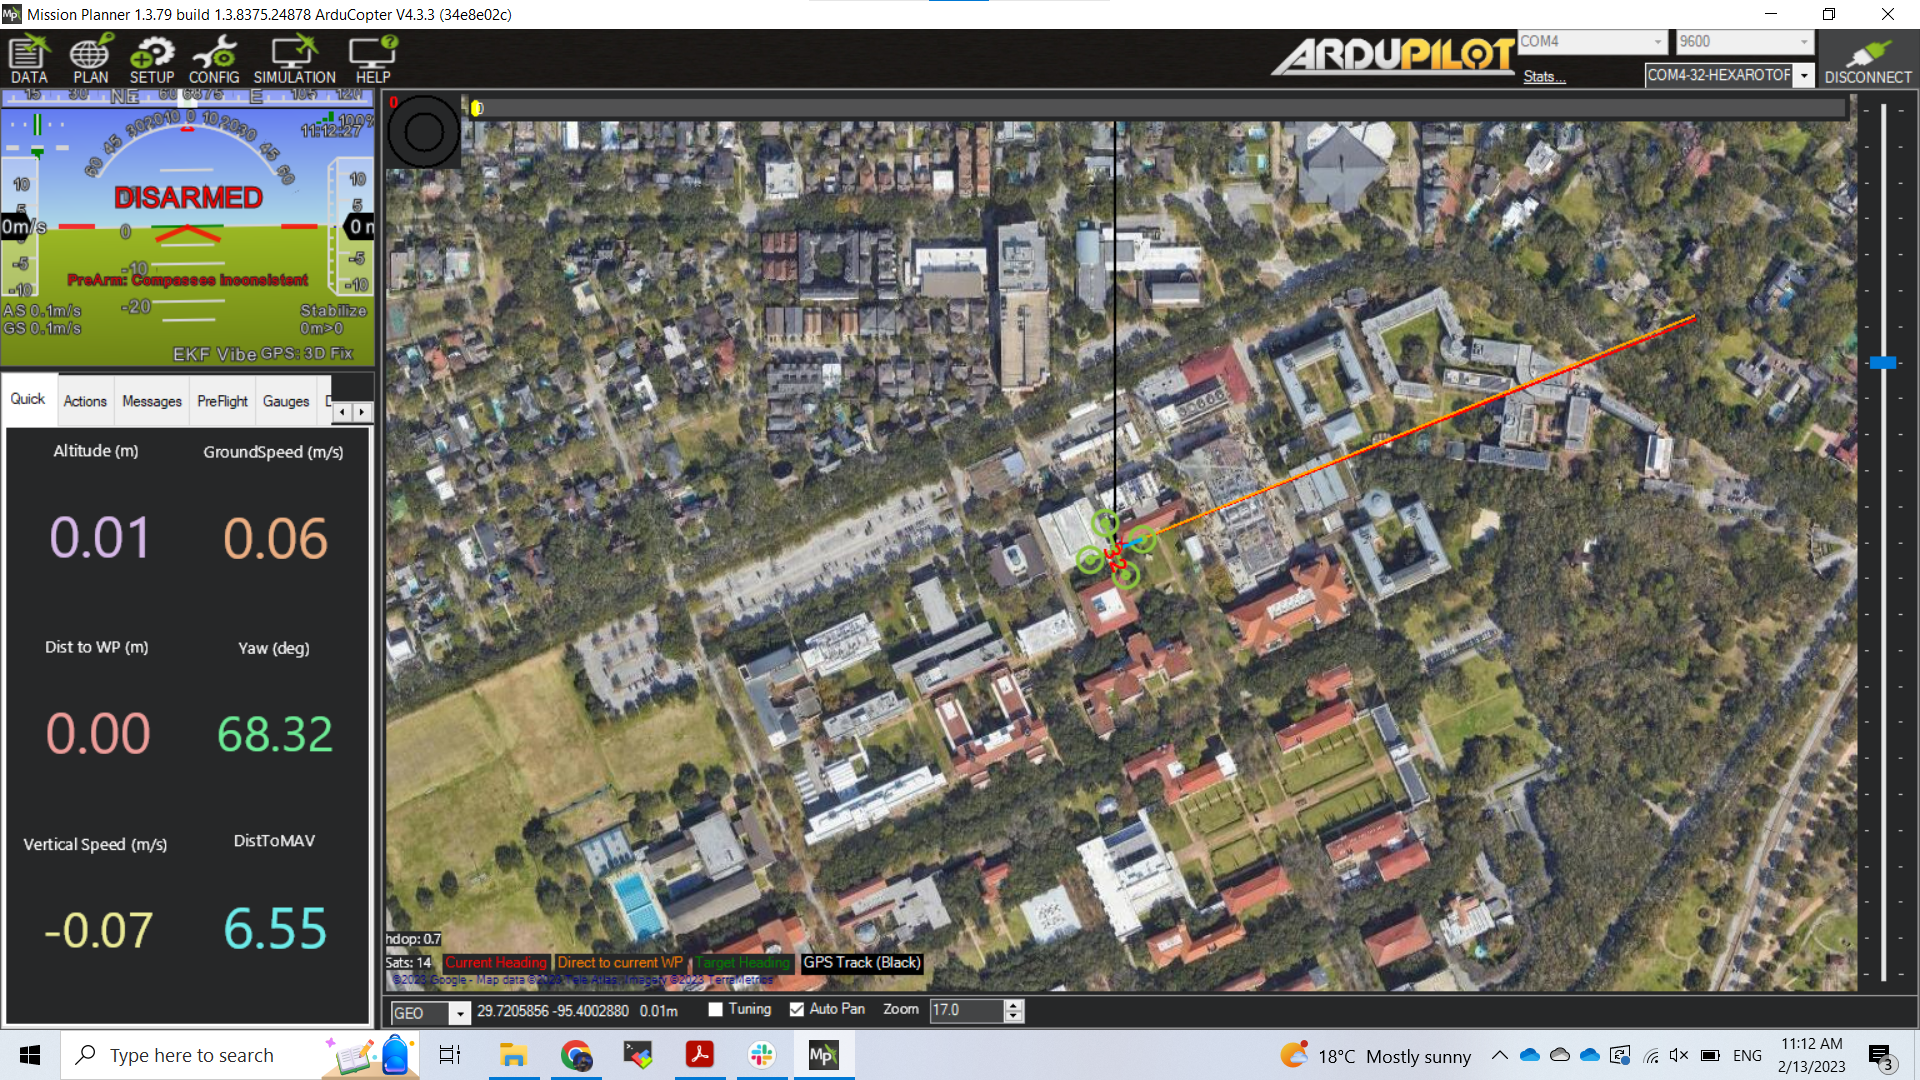
\includegraphics[width=0.5\textwidth]{Figures/Results/Mission_Planner_GUI.png}}
    \caption{Mission Planner GUI Interface.}
    \label{fig3e1}
\end{figure}

Fig.~\ref{fig3e2} shows the real-time status of the drone from SIK Telemetry Radio in Mission Planner GUI. The left side of the image shows the "DISARMED" status, which means the drone is not armed yet, and the right picture shows the "ARMED" status, which means the drone is armed and starts to spin the propellers at a fixed speed.

\begin{figure}[H]
    \centerline{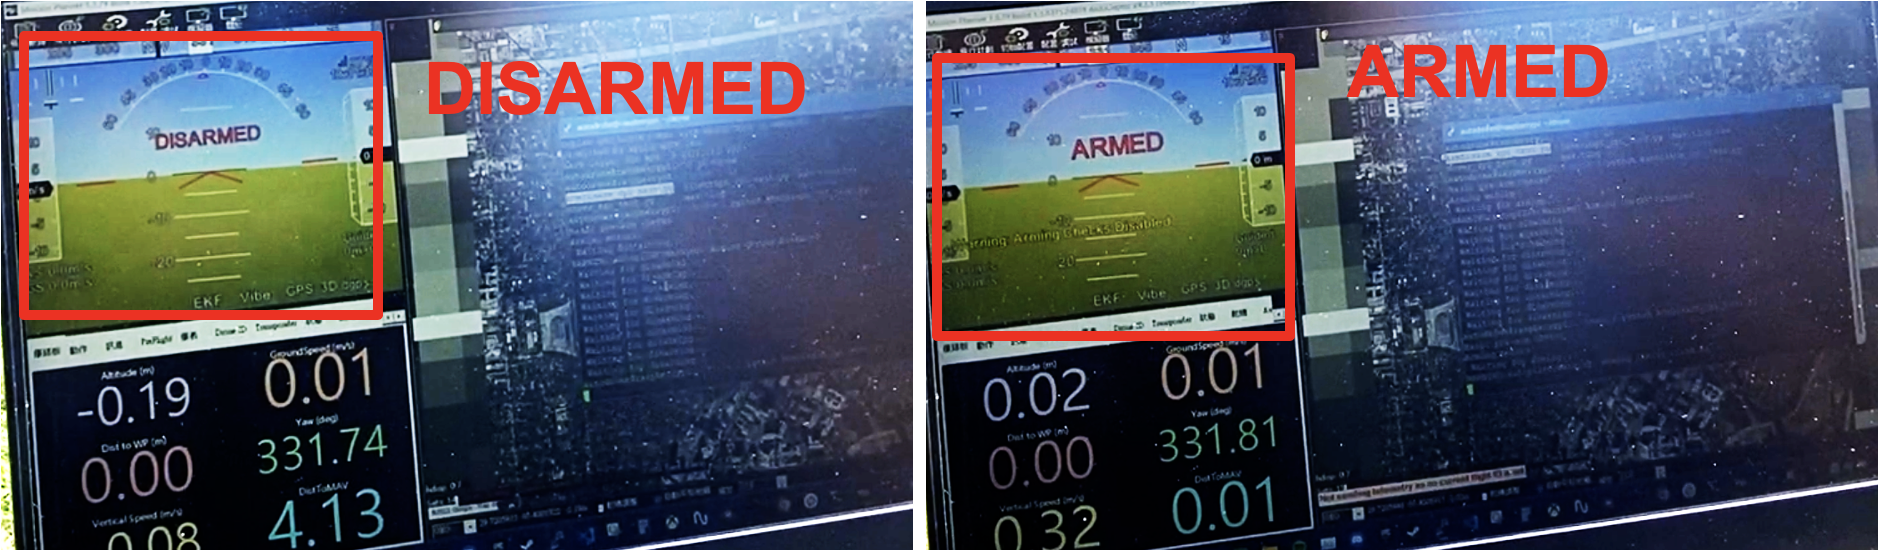
\includegraphics[width=0.5\textwidth]{Figures/Results/GUI_Status.png}}
    \caption{Drone's real-time status on Mission Planner GUI.}
    \label{fig3e2}
\end{figure}